\begin{figure*}[t]
\centering
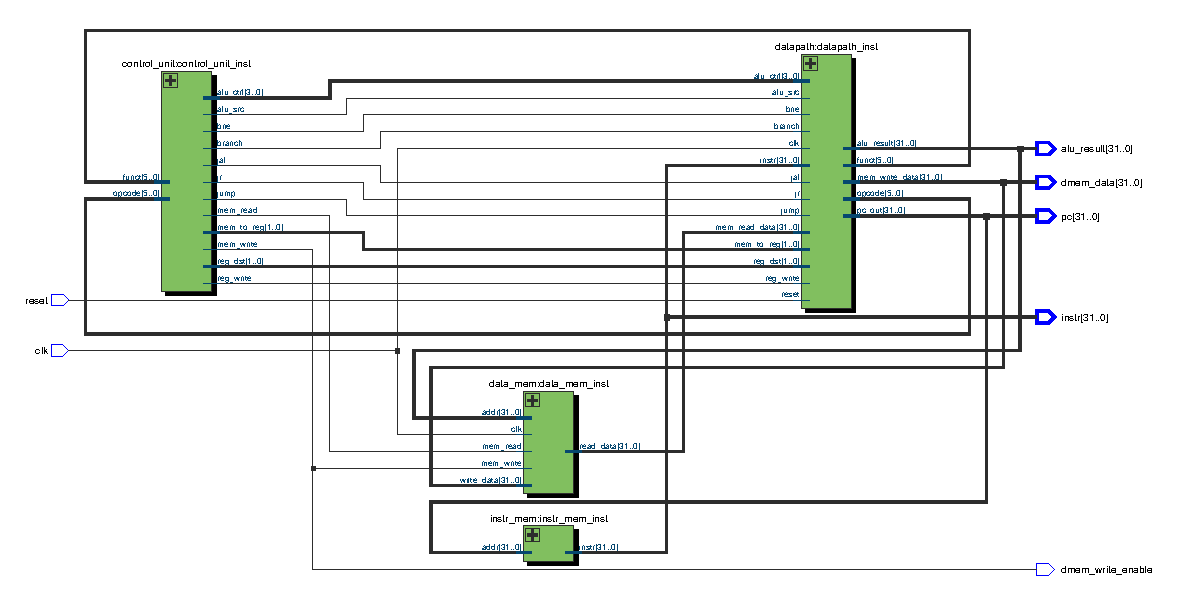
\includegraphics[width=0.95\textwidth]{000-figuras/mips-monociclo.pdf}
\caption{Netlist esquemático estrutural do processador MIPS monociclo no nível de topo (\texttt{mips\_monociclo\_top}) obtido via RTL Viewer no Intel Quartus Prime, evidenciando o modelo Harvard com barramentos desacoplados entre memória de instruções (\texttt{instr\_mem}), memória de dados (\texttt{data\_mem}), unidade de controle (\texttt{control\_unit}) e caminho de dados (\texttt{datapath}).}
\label{fig:rtl_netlist_top}
\end{figure*}

\section{Validação Funcional e Resultados Experimentais}

A metodologia de verificação adotada baseia-se no princípio de que nenhum componente deve ser integrado ao topo hierárquico sem prévia homologação funcional unitária. Foram desenvolvidas 7 bancadas de teste automatizadas com assertivas em Icarus Verilog \cite{icarus_verilog}, além da compilação física no Intel Quartus Prime \cite{intel_quartus_handbook}.

\subsection{Esteira de Automação e Metodologia de Testes}
O fluxo unitário emprega o script \texttt{run\_simulation.sh}, que aciona o simulador Icarus Verilog com suporte ao padrão IEEE 1800-2012 (\texttt{-g2012}) e ativação de avisos (\texttt{-Wall}). Essa rotina assegura a detecção precoce de sinais não conectados.

A execução da suíte completa ocorre pelo script de automação \texttt{run\_all\_tests.sh} via comando \texttt{make test}, compilando os módulos no motor \texttt{vvp}. A Tabela \ref{tab:testes_resumo} consolida os resultados dos 7 módulos com 48 testes e 100\% de aprovação.

\begin{table}[htbp]
\centering
\caption{Consolidado da Suíte de Testes Automatizada (\texttt{make test})}
\label{tab:testes_resumo}
\scriptsize
\setlength{\tabcolsep}{2.5pt}
\begin{tabular}{llcc}
\toprule
\textbf{Módulo} & \textbf{Arquivo} & \textbf{Testes} & \textbf{Status} \\
\midrule
ULA & \texttt{tb\_alu.v} & 11 & Aprovado \\
Datapath Auxiliar & \texttt{tb\_datapath\_aux.v} & 8 & Aprovado \\
Banco de Registradores & \texttt{tb\_reg\_file.v} & 6 & Aprovado \\
Unidade de Controle & \texttt{tb\_control\_unit.v} & 13 & Aprovado \\
Memória de Instruções & \texttt{tb\_instr\_mem.v} & 5 & Aprovado \\
Memória de Dados & \texttt{tb\_data\_mem.v} & 4 & Aprovado \\
Top-Level com Sort & \texttt{tb\_mips\_monociclo\_top.v} & 1 & Aprovado \\
\midrule
\textbf{Total da Suíte} & \textbf{7 Arquivos} & \textbf{48} & \textbf{100\% (0 erros)} \\
\bottomrule
\end{tabular}
\end{table}

\subsection{Alvos de Verificação dos Módulos Unitários}
Cada bancada de teste foi projetada com alvos de homologação específicos:

\begin{itemize}\setlength{\itemsep}{2pt}\setlength{\parskip}{0pt}
    \item \textbf{ULA (\texttt{tb\_alu.v})}: validou operações lógicas AND, OR e NOR, adições e subtrações com inteiros positivos e negativos em complemento a dois, ativação da linha de zero em resultado nulo, comparações de magnitude com sinal via \texttt{\$signed} e deslocamento lógico \texttt{sll} com controle de deslocamento via \texttt{shamt};
    \item \textbf{Datapath Auxiliar (\texttt{tb\_datapath\_aux.v})}: comprovou o sincronismo do registrador de PC com reset síncrono, os somadores dedicados de $\text{PC}+4$ e de branch com cálculo de deslocamento relativo, multiplexadores de seleção de barramentos e extensão de sinal com preservação do bit de magnitude;
    \item \textbf{Banco de Registradores (\texttt{tb\_reg\_file.v})}: verificou a concorrência de leitura assíncrona em duas portas simultâneas, escrita síncrona habilitada por \texttt{reg\_write} e blindagem inviolável do registrador \$0, rejeitando tentativas de sobrescrita;
    \item \textbf{Unidade de Controle (\texttt{tb\_control\_unit.v})}: testou a decodificação exata de instruções Tipo-R, Tipo-I e Tipo-J, os sinais de controle de memória e desvio, além da trava combinacional que inibe o sinal \texttt{reg\_write} na instrução \texttt{jr};
    \item \textbf{Memória de Instruções (\texttt{tb\_instr\_mem.v})}: validou a leitura sequencial das instruções compiladas do arquivo \texttt{sort.bin} e a máscara de endereçamento \texttt{addr[9:2]} para contornar o offset virtual do simulador MARS;
    \item \textbf{Memória de Dados (\texttt{tb\_data\_mem.v})}: homologou escritas síncronas na borda de subida do clock com \texttt{mem\_write}, leituras assíncronas com \texttt{mem\_read} e isolamento de palavras adjacentes.
\end{itemize}

\subsection{Resultados da Integração Top-Level e Ordenação}
O teste definitivo da microarquitetura consistiu na execução do programa de ordenação canônico de Patterson e Hennessy \cite{patterson_mips} sobre o processador completo.

No início da simulação injetou-se na memória RAM um vetor de 5 elementos desordenados nas posições \texttt{ram[0]} a \texttt{ram[4]}. O processador operou de forma autônoma ao longo de 5000 ns de simulação, percorrendo laços de repetição, efetuando comparações e executando chamadas à sub-rotina de troca com \texttt{jal} e \texttt{jr}. A Tabela \ref{tab:ram_sort} exibe o estado físico das células de memória antes e depois da execução.

\begin{table}[htbp]
\centering
\caption{Estado da Memória de Dados (RAM) Antes e Após o Sort}
\label{tab:ram_sort}
\scriptsize
\setlength{\tabcolsep}{4pt}
\begin{tabular}{ccccc}
\toprule
\textbf{Índice} & \textbf{Endereço} & \textbf{Inicial} & \textbf{Final} & \textbf{Posição} \\
\midrule
\texttt{ram[0]} & \texttt{0x00} & 88 & \textbf{7}  & Mínimo \\
\texttt{ram[1]} & \texttt{0x04} & 15 & \textbf{15} & 2$^\circ$ menor \\
\texttt{ram[2]} & \texttt{0x08} & 42 & \textbf{42} & Mediano \\
\texttt{ram[3]} & \texttt{0x0C} & 7  & \textbf{88} & 4$^\circ$ elemento \\
\texttt{ram[4]} & \texttt{0x10} & 99 & \textbf{99} & Máximo \\
\bottomrule
\end{tabular}
\end{table}

A transição do vetor de $[88, 15, 42, 7, 99]$ para a sequência ordenada $[7, 15, 42, 88, 99]$ comprova a integridade funcional do caminho de dados e da unidade de controle. A Fig. \ref{fig:top_output} exibe o log de execução do terminal.

\begin{figure}[htbp]
\centering
\begin{lstlisting}[style=estiloTerminal]
[ANTES]  RAM: [88, 15, 42, 7, 99]
[DEPOIS] RAM: [7, 15, 42, 88, 99]
>>> TESTE DO SORT CONCLUIDO COM SUCESSO! <<<
\end{lstlisting}
\caption{Log da simulação do processador executando o algoritmo Sort.}
\label{fig:top_output}
\end{figure}

\subsection{Validação Física e Síntese no Intel Quartus Prime}
Para comprovar que a descrição em Verilog HDL representa um circuito realizável em silício e não apenas uma simulação abstrata, o projeto foi submetido ao fluxo completo de compilação física no Intel Quartus Prime \cite{intel_quartus_handbook} voltado ao FPGA Intel MAX 10 modelo \texttt{10M50DAF484C7G} da placa DE10-Lite \cite{terasic_de10_lite_user_manual}.

O fluxo de compilação física via \texttt{make quartus-build} articula as seguintes etapas:
\begin{enumerate}\setlength{\itemsep}{1pt}\setlength{\parskip}{0pt}
    \item \texttt{quartus\_map}: executou a análise sintática, elaboração hierárquica e síntese lógica dos 15 módulos HDL, mapeando o circuito em 17.089 elementos lógicos (LEs);
    \item \texttt{quartus\_fit}: realizou o posicionamento e roteamento físico nas matrizes de interconexão do chip com ocupação média de 15\% dos recursos de roteamento. A ferramenta promoveu automaticamente os sinais \texttt{clk} e \texttt{reset} para as redes de clock globais dedicadas \texttt{CLKCTRL\_G3} e \texttt{CLKCTRL\_G4}, eliminando distorções de fase (\textit{skew}) e prevenindo violações temporais;
    \item \texttt{quartus\_asm}: gerou o arquivo de programação binária \texttt{mips\_monociclo.sof} com contagem nula de erros.
\end{enumerate}

A Tabela \ref{tab:quartus_resumo} consolida as métricas da implementação física, cujo netlist sintetizado é detalhado na Fig. \ref{fig:rtl_netlist_top}. A inspeção estrutural no RTL Viewer confirmou a ausência total de latches espúrios na ULA, nos multiplexadores e na unidade de controle, comprovando conformidade com as regras de projeto síncrono para lógica reconfigurável.

\begin{table}[htbp]
\centering
\caption{Métricas da Síntese Física no Intel Quartus Prime}
\label{tab:quartus_resumo}
\scriptsize
\setlength{\tabcolsep}{3pt}
\begin{tabular}{ll}
\toprule
\textbf{Métrica de Hardware} & \textbf{Resultado Obtido} \\
\midrule
Dispositivo Alvo & Intel MAX 10 (\texttt{10M50DAF484C7G}) \\
Elementos Lógicos (LEs) & 17.089 células lógicas \\
Pinos de Entrada/Saída & 131 pinos (2 entradas, 129 saídas) \\
Redes Globais de Relógio & 2 (\texttt{CLKCTRL\_G3} e \texttt{CLKCTRL\_G4}) \\
Taxa de Roteamento (Interconnect) & 15\% média (75\% pico regional) \\
Latches Transparentes Espúrios & 0 inferidos (circuito 100\% síncrono) \\
Bitstream de Programação & \texttt{mips\_monociclo.sof} (0 erros) \\
\bottomrule
\end{tabular}
\end{table}

A prevenção de latches espúrios constitui um dos critérios mais rigorosos no projeto de circuitos digitais sintetizáveis. Em descrições comportamentais com blocos \texttt{always @(*)}, a omissão involuntária de ramos condicionais em cláusulas \texttt{case} ou \texttt{if/else} induz a ferramenta a inferir elementos de memória transparentes assíncronos, degradando a confiabilidade do circuito. A análise do log de síntese confirmou cobertura exaustiva de ramos nas matrizes de decodificação de controle e multiplexação, assegurando lógica puramente combinacional.

No estágio de roteamento (\texttt{quartus\_fit}), o compilador promoveu os sinais \texttt{clk} e \texttt{reset} às linhas de distribuição de baixa impedância \texttt{CLKCTRL\_G3} e \texttt{CLKCTRL\_G4}. Essa atribuição minimiza distorções de fase (\textit{clock skew}) sobre os 32 registradores e o contador de programa. A geração do bitstream binário \texttt{mips\_monociclo.sof} comprova a prontidão do hardware para execução física imediata na placa DE10-Lite via comando \texttt{make quartus-pgm}.
